\begin{figure}[H]
    \centering
    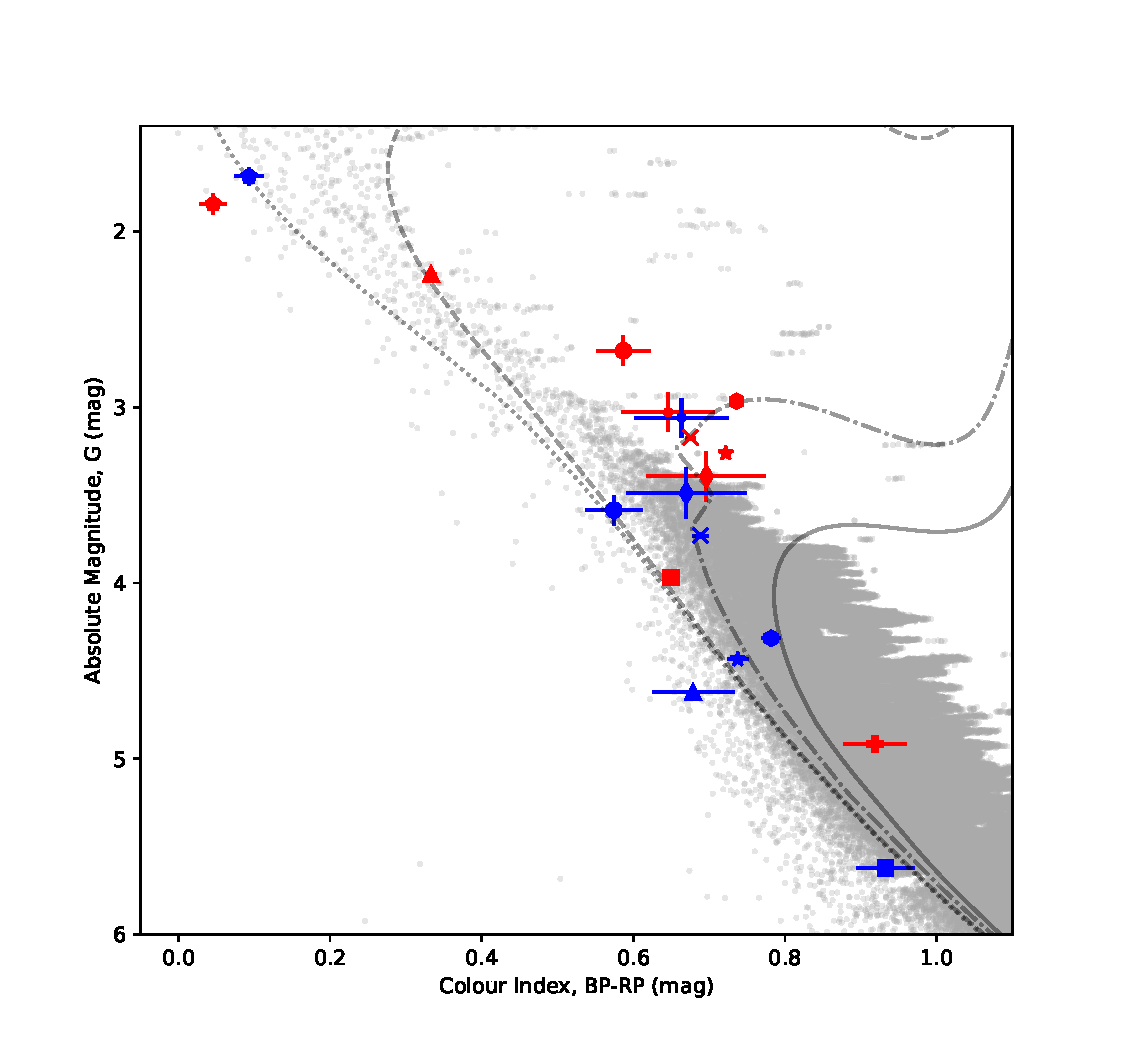
\includegraphics[width=\linewidth]{HRD}
    \caption{The two colours, red and blue, represent primary and secondary components respectively. These symbols represent EBs: TIC279087522 ($\pentagonblack$), TIC30122338 ($\mdblkcircle$), TIC7695666 ($\times$), TIC66602813 ($\mdblksquare$), TIC63579446 ($\bigstar$), TIC201497357 ($\blacktriangle)$, TIC349480507 ($\cdot$), TIC349059354 ($\mdblkdiamond$), TIC78568736 ($+$; secondary outside figure boundaries), TIC80556181 ($\varhexagonblack$). Isochrones from \citet{Dotter16,Choi16,Paxton18} represent stellar ages $0.5 - 10 \mathrm{\ Gyr}$ from left to right. Main sequence stars (grey) are from \citet{Gaia18}}.
    \label{fig:CMD}
\end{figure}